
\documentclass[]{article}

\title{Retroalimentación de propuestas para proyecto final}

\date{}
\usepackage{braket}
\usepackage{bbold}
\usepackage{amsmath,amsfonts,amssymb,amsthm,booktabs}
\usepackage[margin=1.0in]{geometry}
\usepackage{graphicx}
\usepackage{chngcntr}
\usepackage{floatrow}
\usepackage{chngcntr}
\usepackage{hyperref}
\usepackage[spanish]{babel}
\usepackage[svgnames]{xcolor}
\usepackage{commath}
\usepackage{floatrow}
\usepackage{pdfpages}


\DeclareMathOperator{\EX}{\mathbb{E}}% expected val
\renewcommand{\spanishtablename}{Cuadro}
\usepackage{listings}
\usepackage[%
    font={small,sf},
    labelfont=bf,
    format=hang,    
    format=plain,
    margin=0pt,
    width=0.8\textwidth,
]{caption}
\usepackage[list=true]{subcaption}
\lstset{language=R,
    basicstyle=\small\ttfamily,
    stringstyle=\color{DarkGreen},
    otherkeywords={0,1,2,3,4,5,6,7,8,9},
    morekeywords={TRUE,FALSE},
    deletekeywords={data,frame,length,as,character},
    keywordstyle=\color{blue},
    commentstyle=\color{DarkGreen},
}

\begin{document}
%\newpage
\thispagestyle{empty}
\vspace{10 cm}
\begin{scshape}
\begin{center}
	{$\,$} \\[20 mm]
	{\Large{Universidad Autónoma de Nuevo León}} \\[5mm]
	{\large{Facultad de Ingeniería Mecánica y Eléctrica}} \\[5mm]
	{\large{M. C. DE LA ING. OR. SISTEMAS}} \\[5 mm]
	{\large{Maestría}}
	\vskip16mm
	\begin{figure}[h!]
		\centering
		\begin{subfigure}{0.3\linewidth}
			
\includegraphics[width=\linewidth]{Figuras/uanl}
		\end{subfigure}
		\hspace{15 mm}
		\begin{subfigure}{0.2\linewidth}
			
\includegraphics[width=\linewidth]{Figuras/fime}
		\end{subfigure}
	\end{figure}
	\vskip16mm
	\begin{tabular}{p{11cm}}
		\centering
		{\large Portafolio de Evidencias}
	\end{tabular}
	\vskip7mm
	{de}\\[7mm]
	{\large Joaquin Arturo Velarde Moreno}\\[3mm]
	{1649290}\\[7 mm]
	{para el curso de Modelos Probabilistas Aplicados,}\\[3mm]
	{con la profesora Satu Elisa Schaeffer.}\\[3mm]
	Semestre Agosto 2020 - Enero 2021. \\ [5 mm]
	\url{https://github.com/joaquin3600/Modelos_Probabilistas_Aplicados}
	\vfill
\end{center}
\end{scshape}
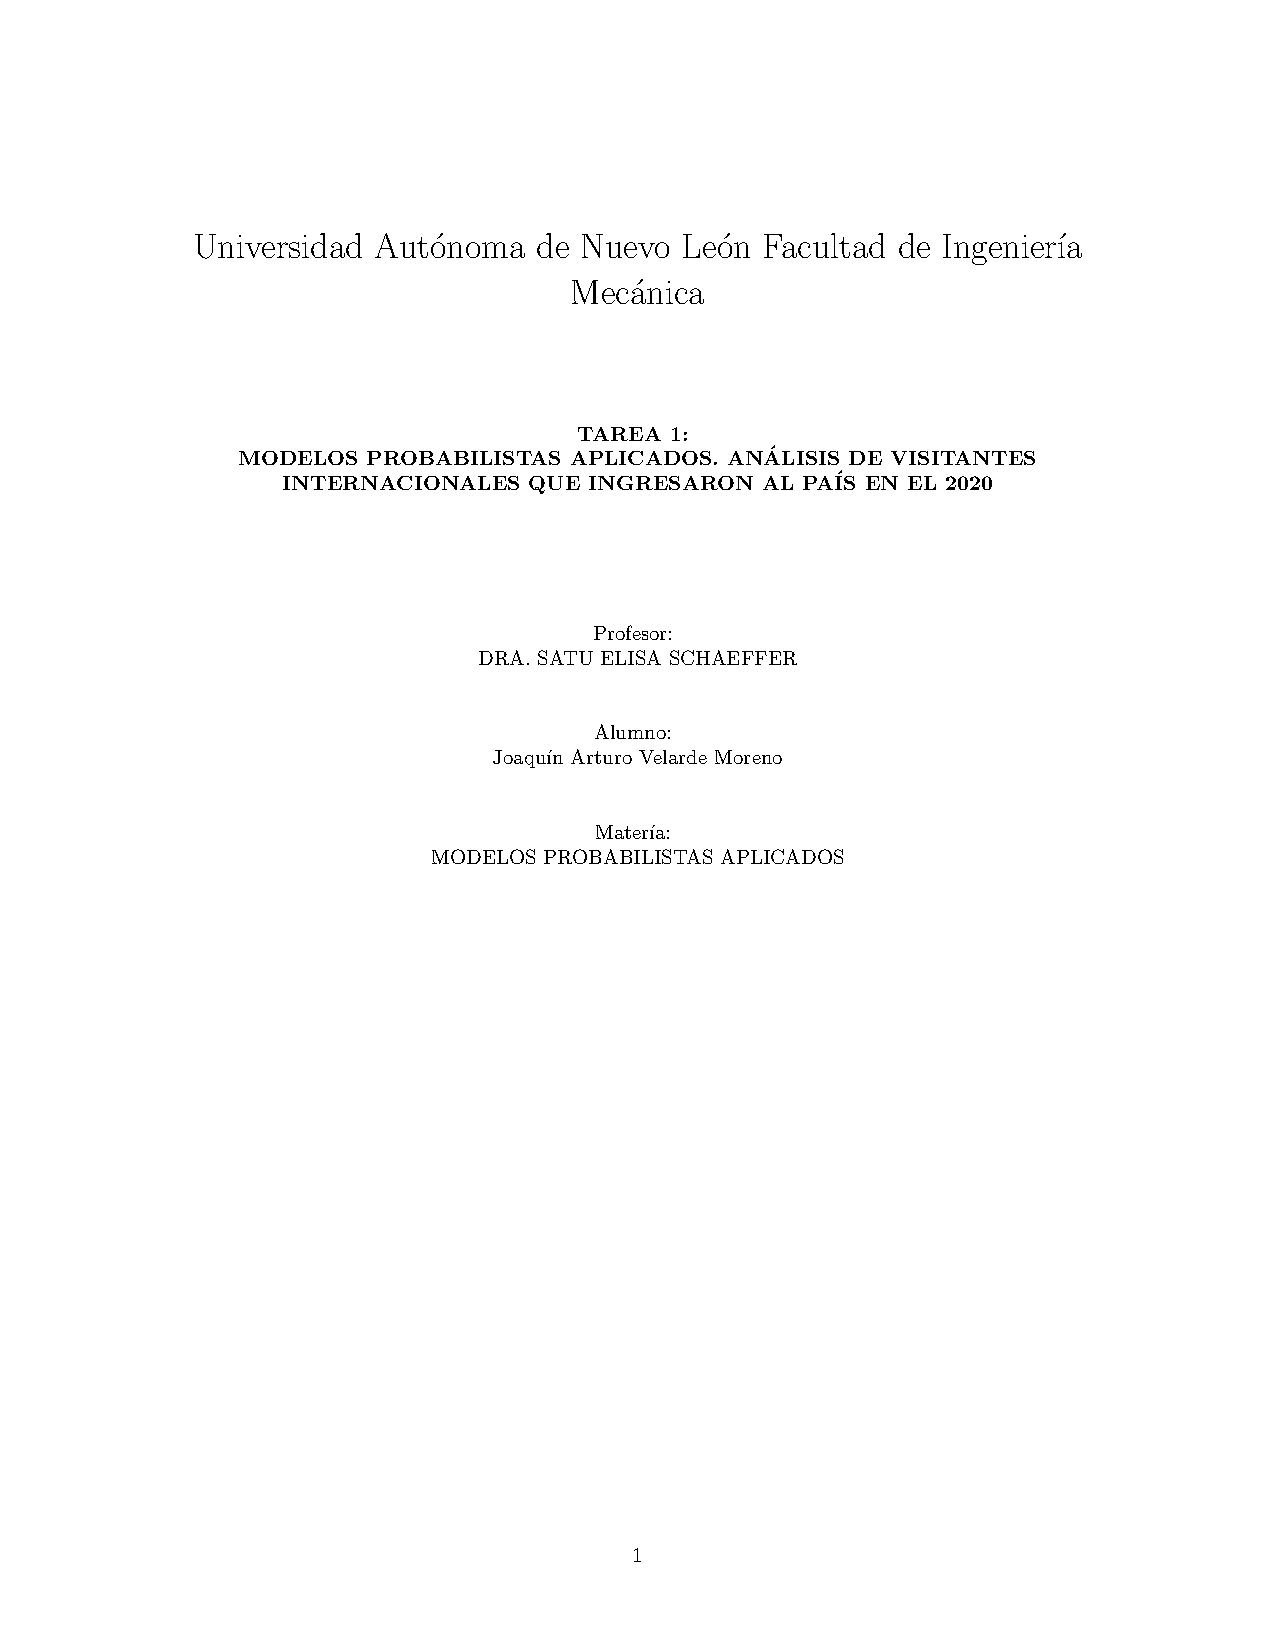
\includepdf[pages=-]{Tareas/Reporte_1.pdf}

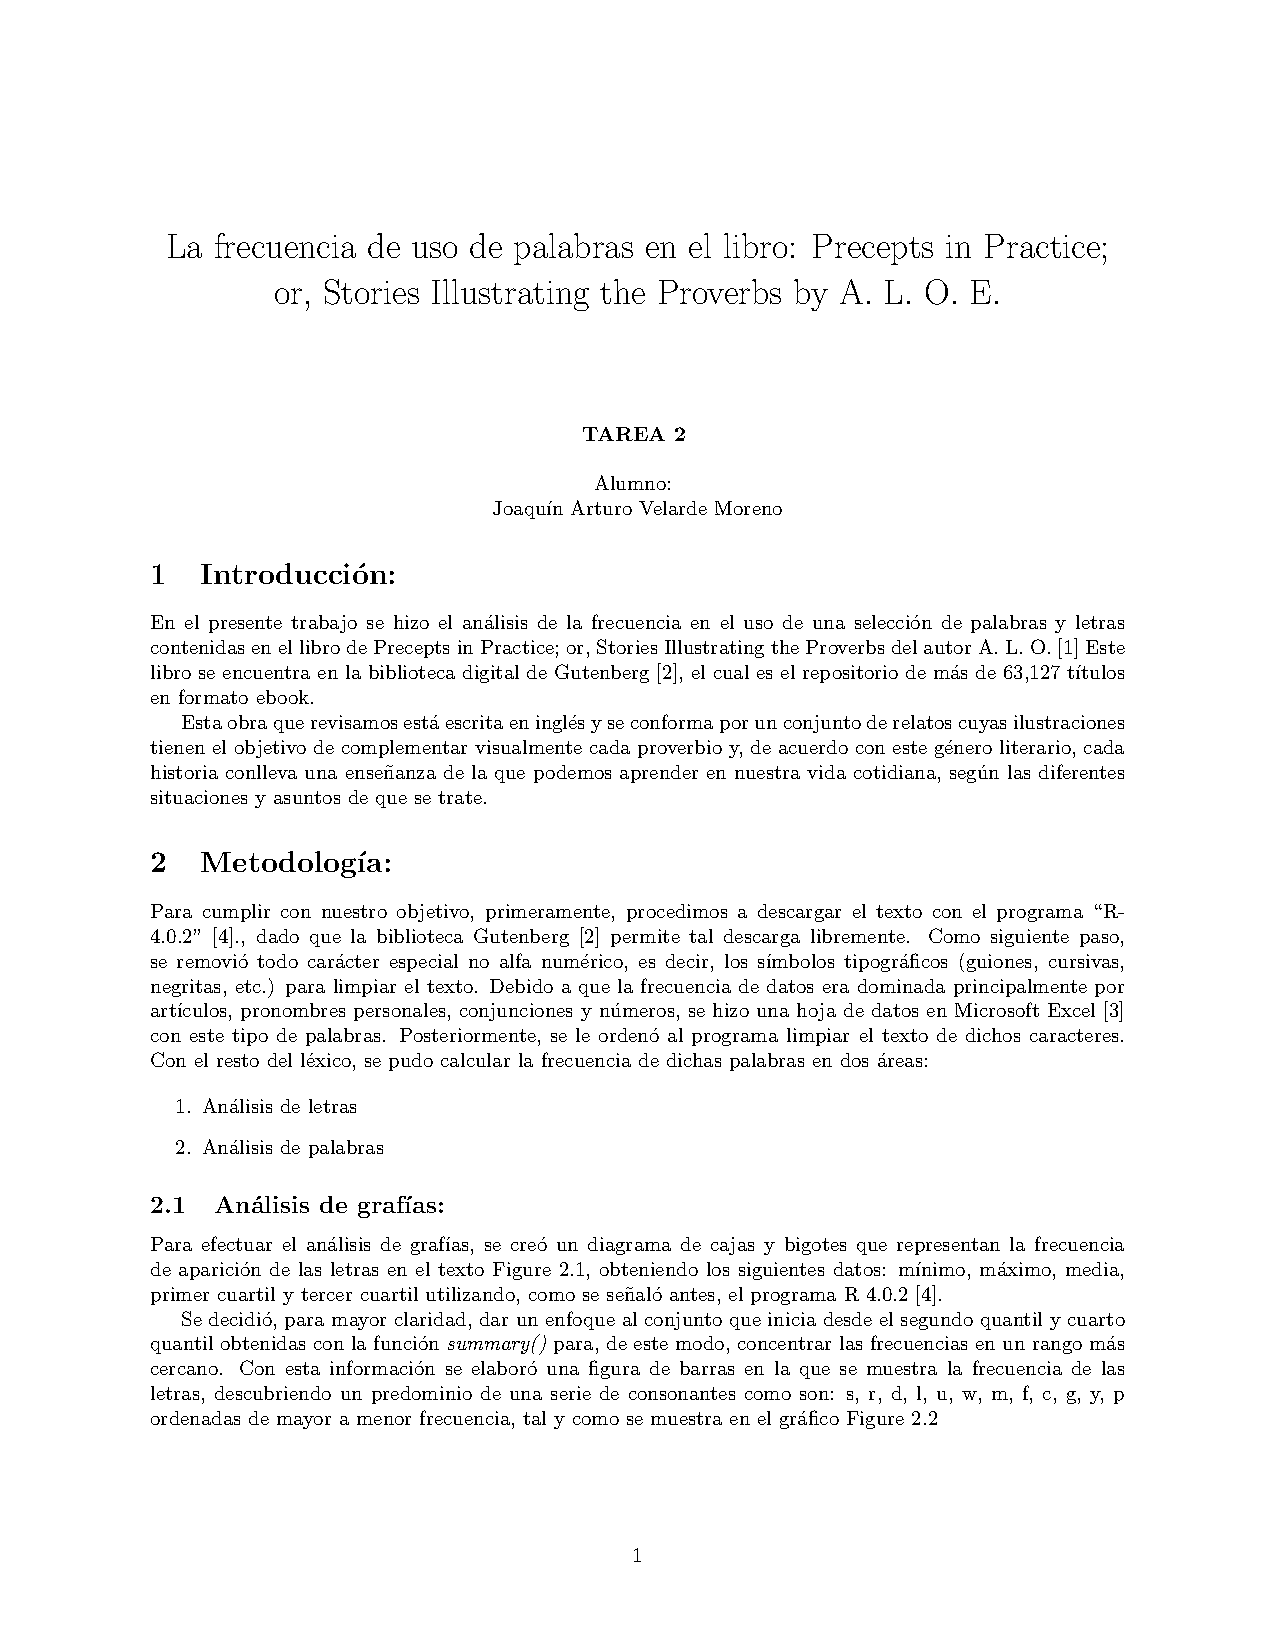
\includepdf[pages=-]{Tareas/Reporte_2.pdf}

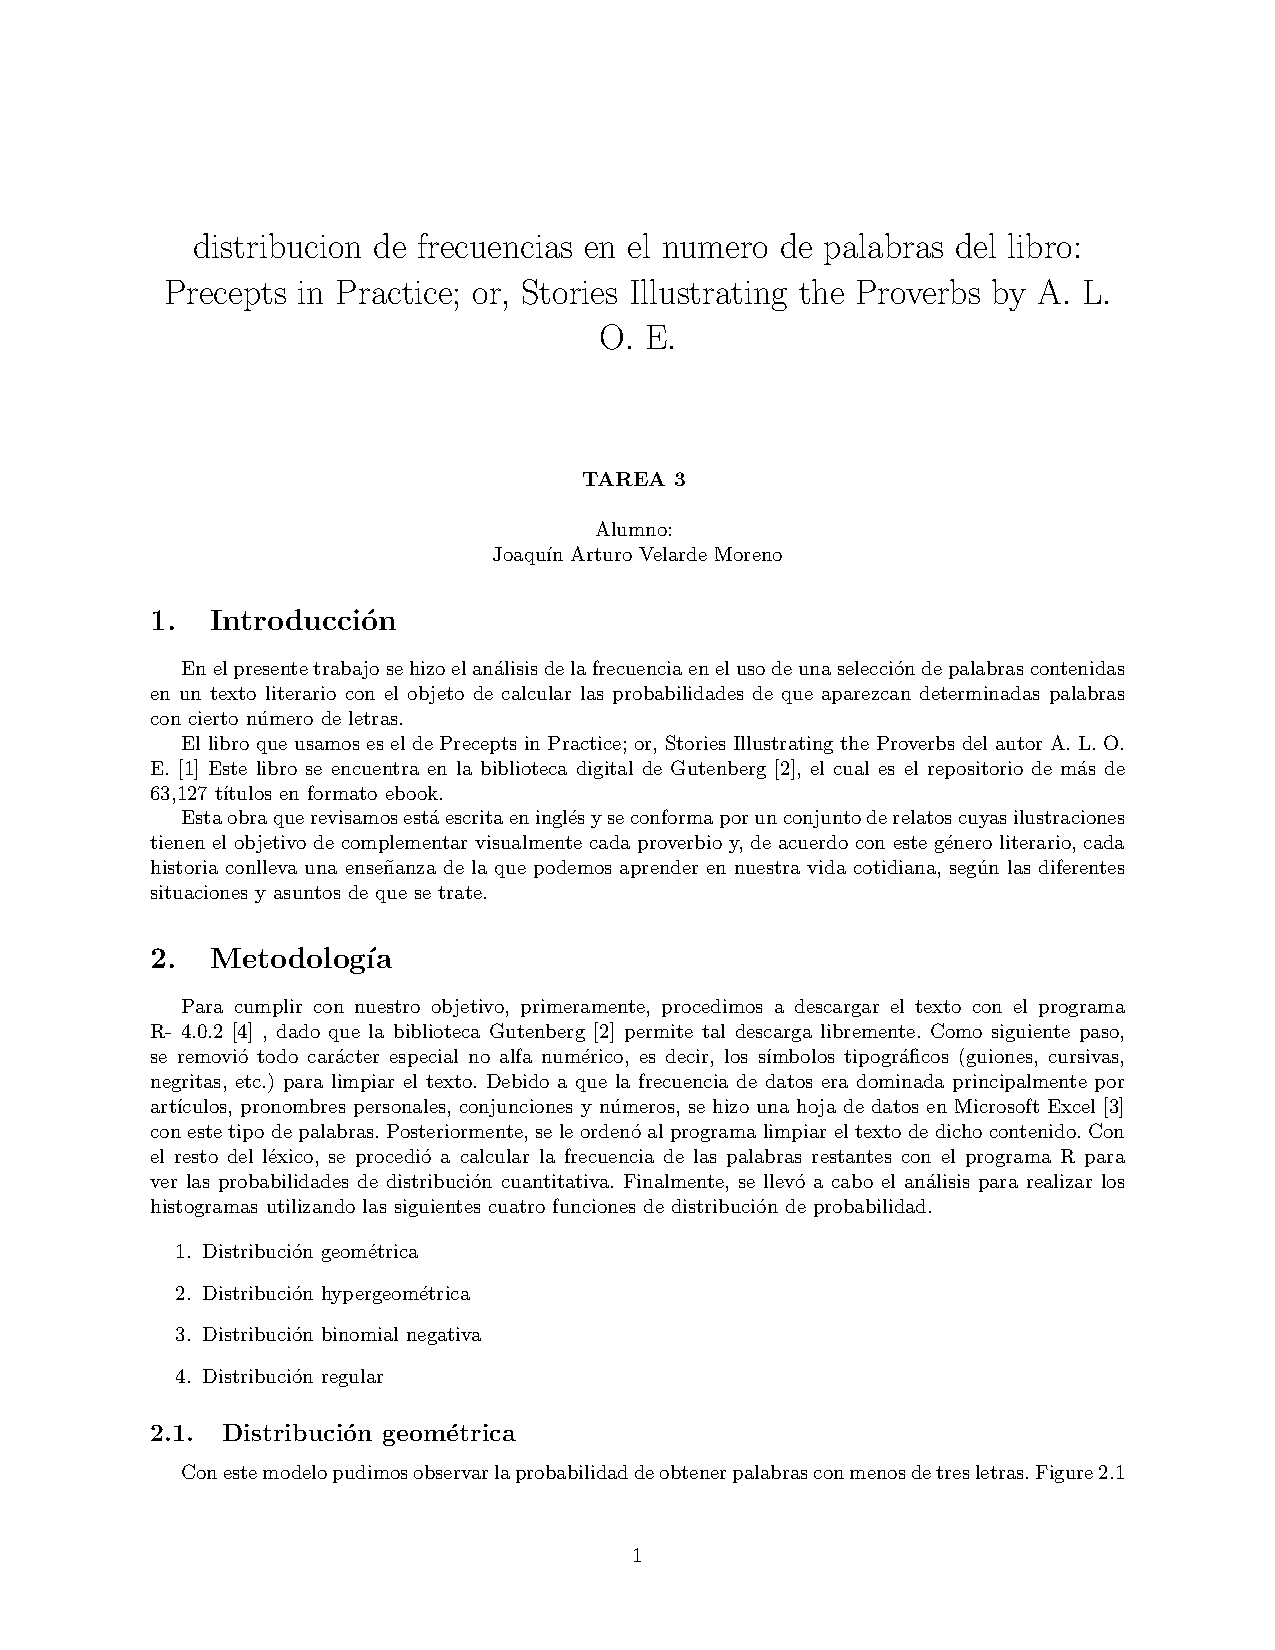
\includepdf[pages=-]{Tareas/Reporte_3.pdf}

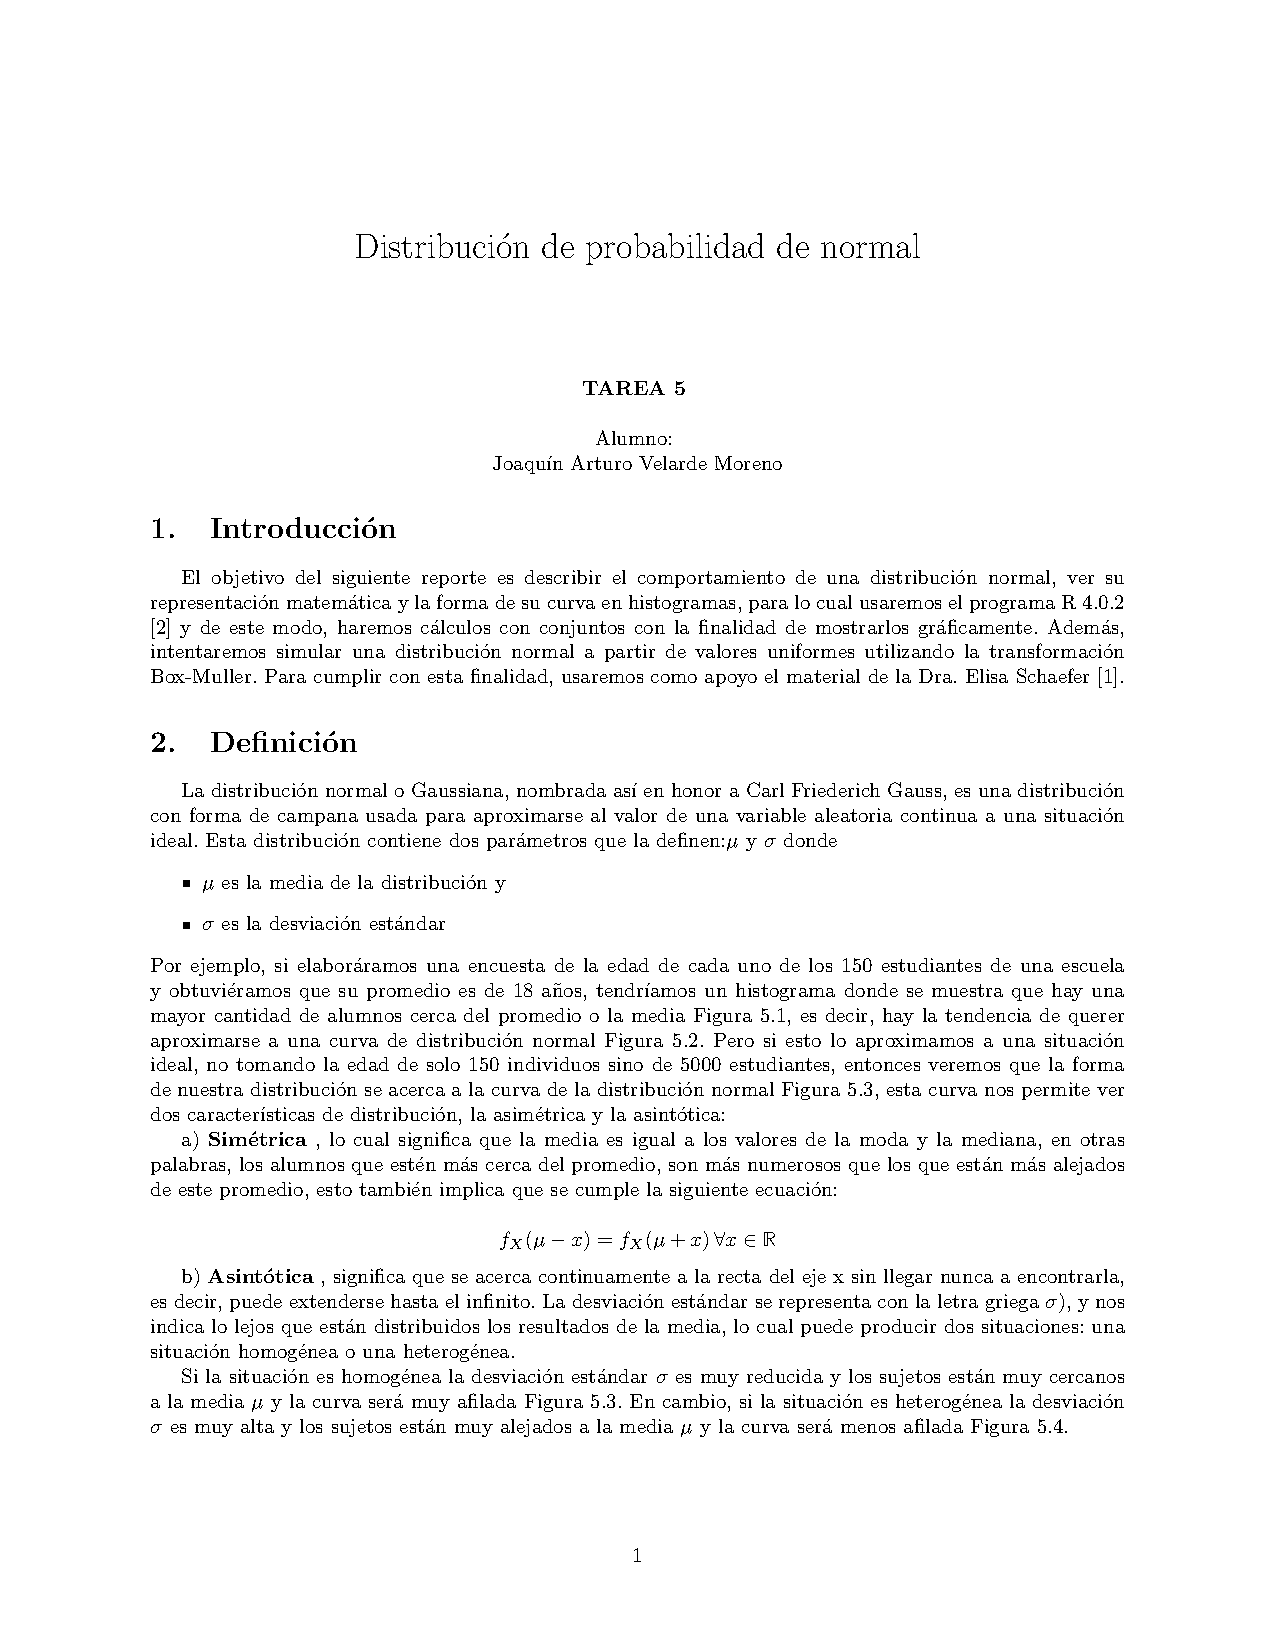
\includepdf[pages=-]{Tareas/Reporte_5.pdf}

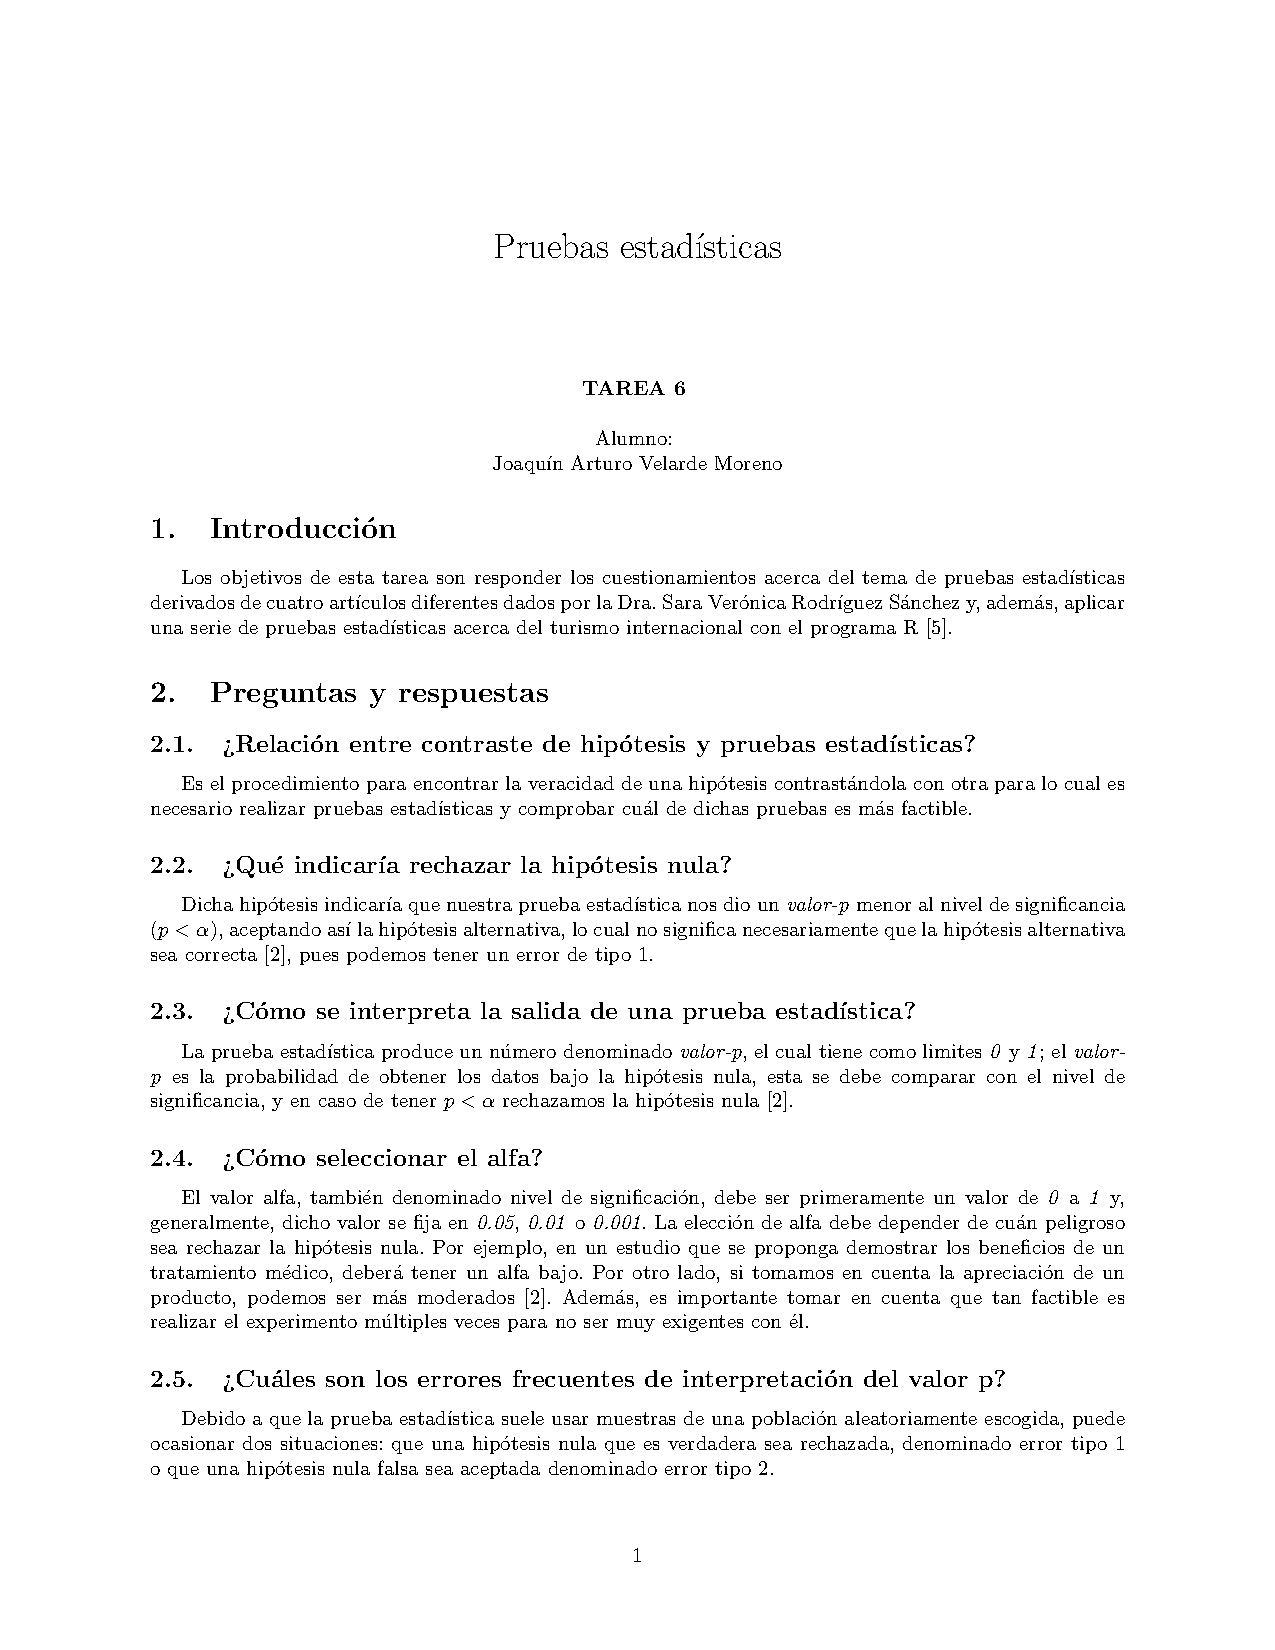
\includepdf[pages=-]{Tareas/Reporte_6.pdf}

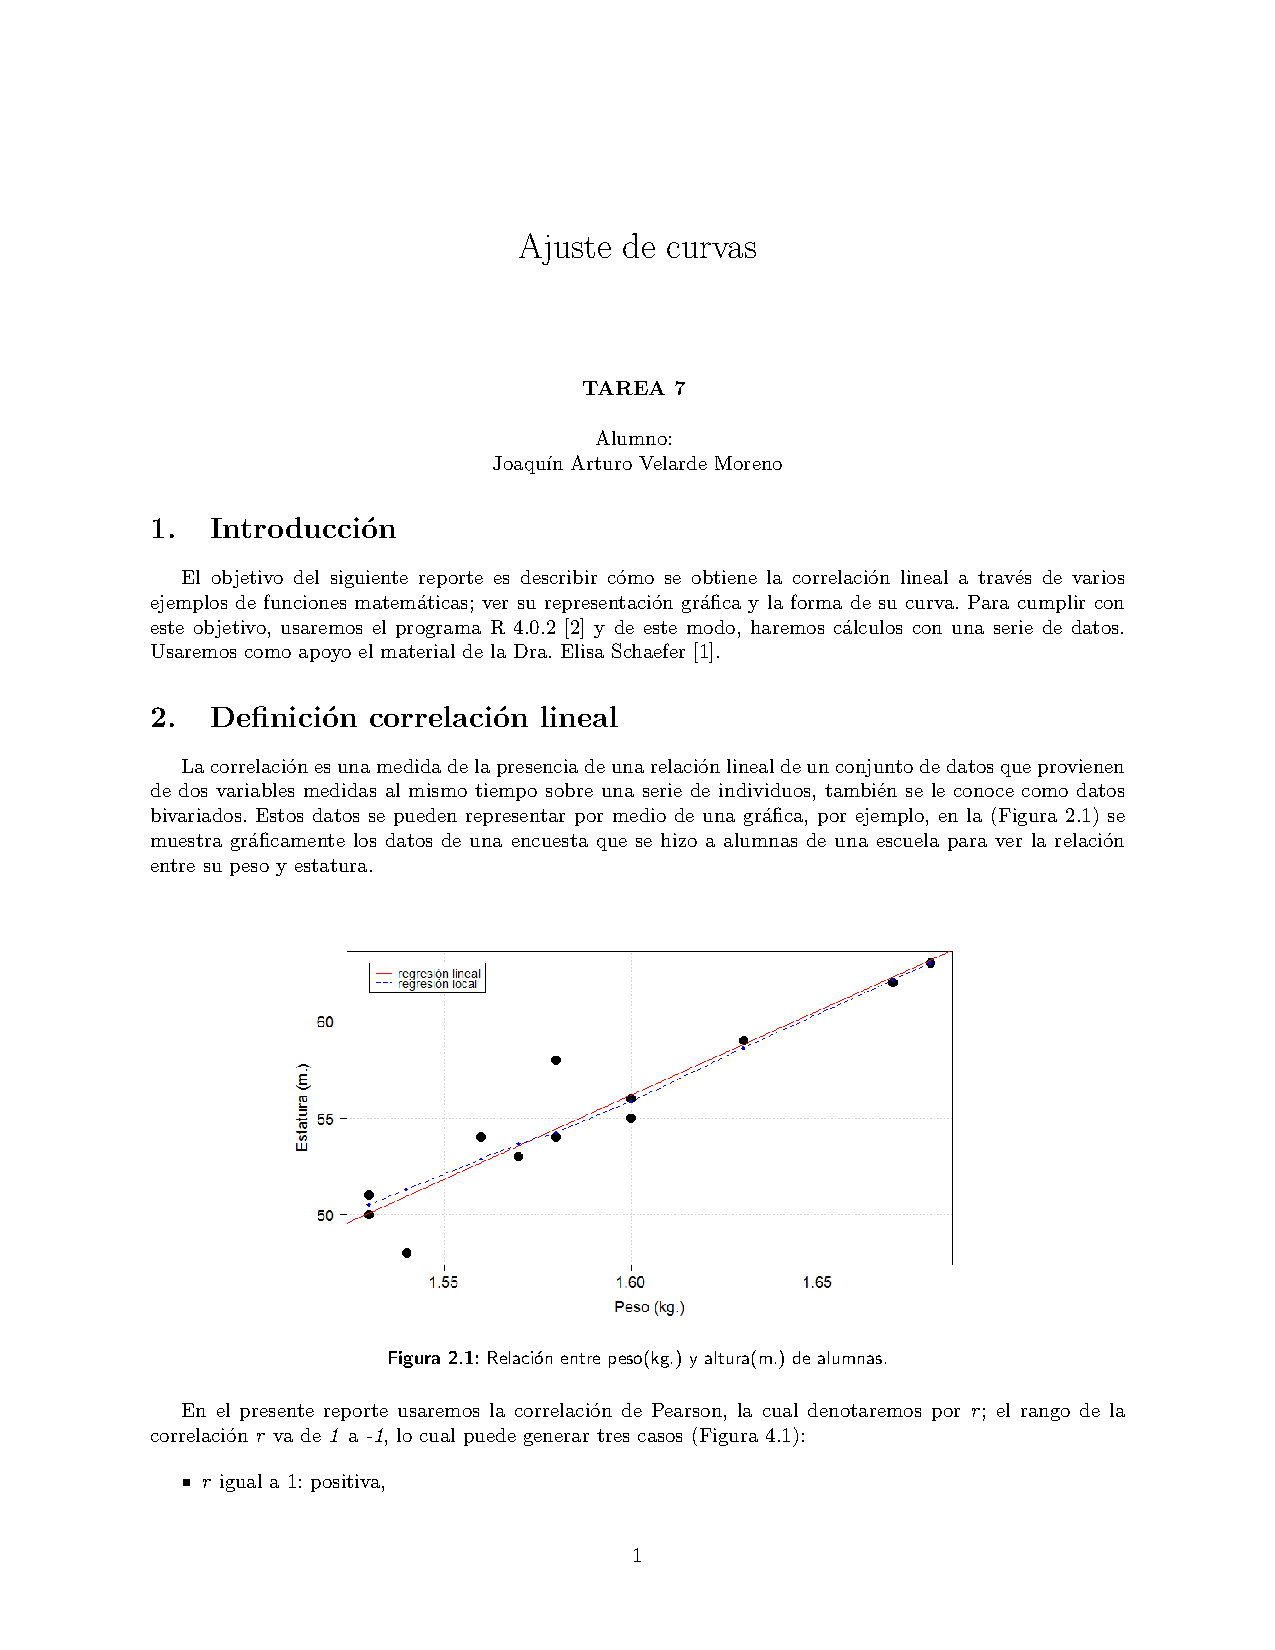
\includepdf[pages=-]{Tareas/Reporte_7.pdf}

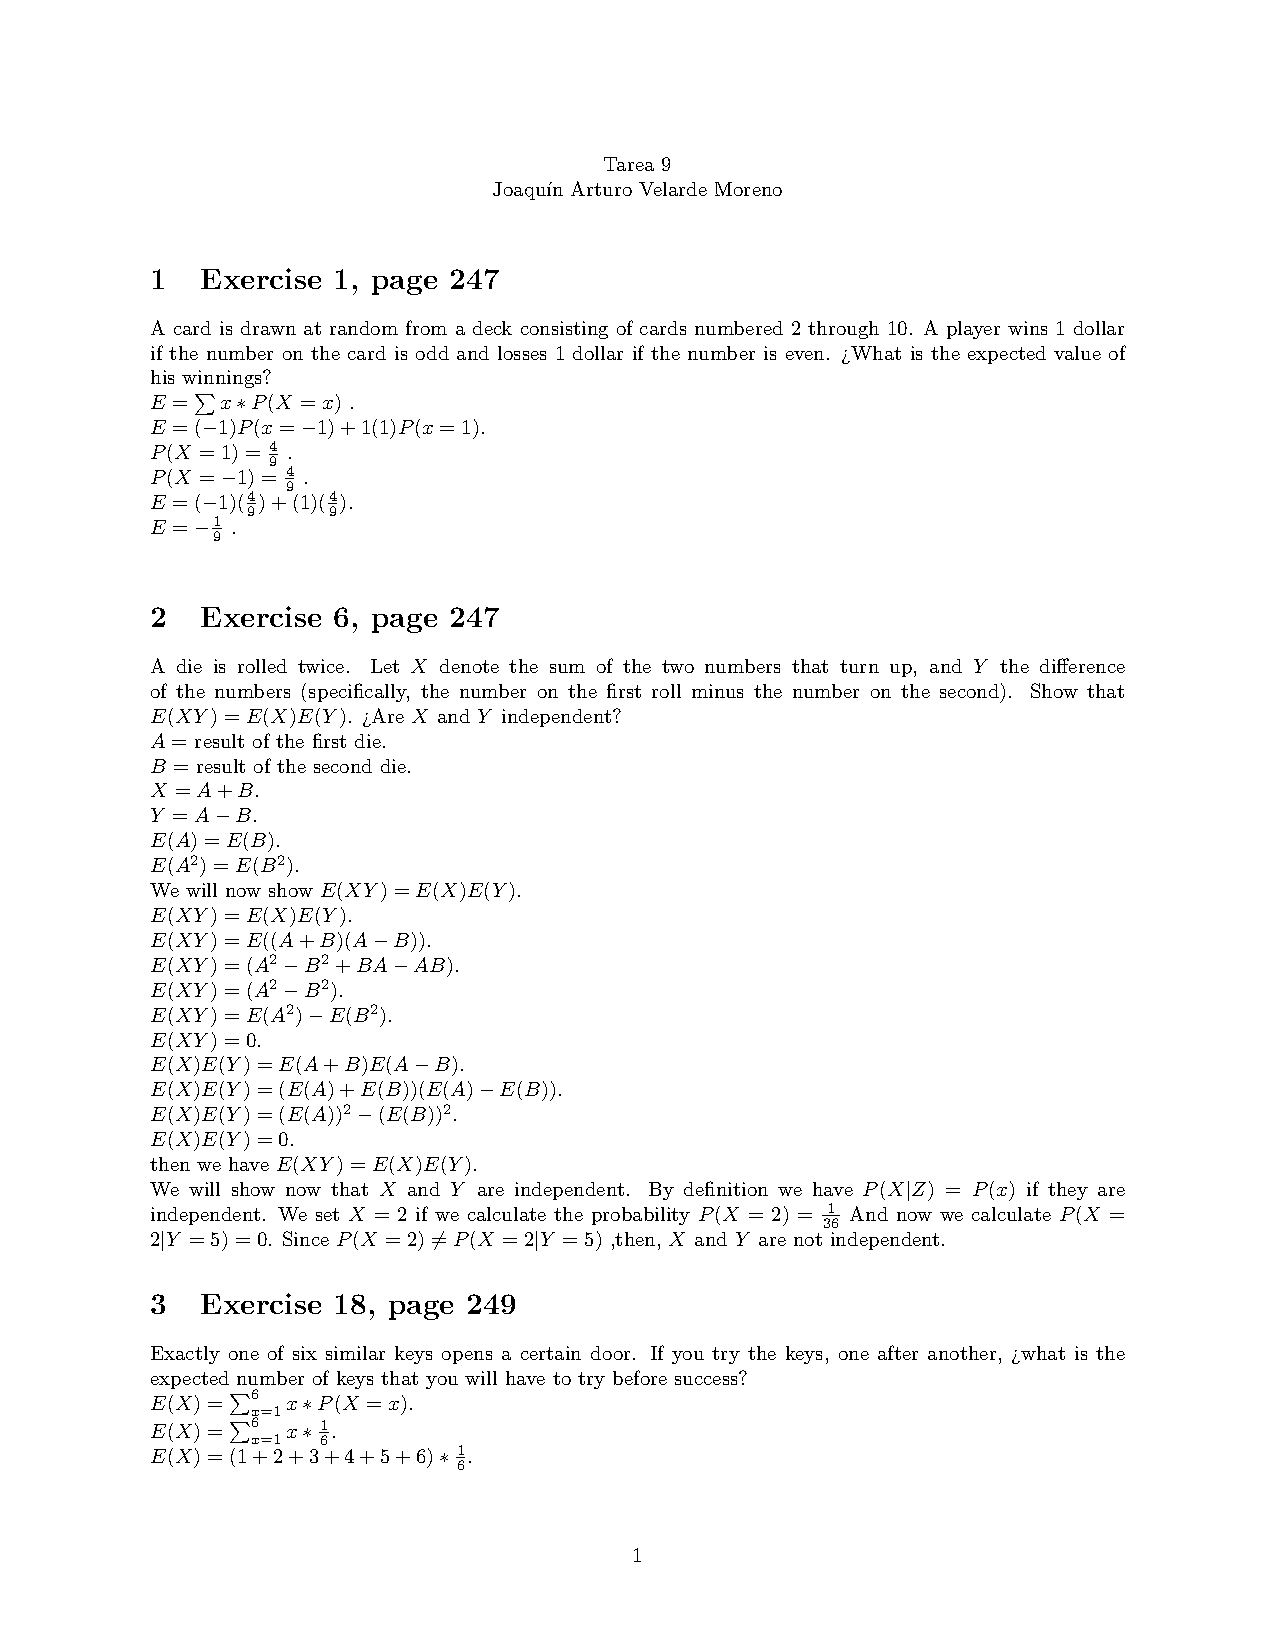
\includepdf[pages=-]{Tareas/Reporte_9.pdf}

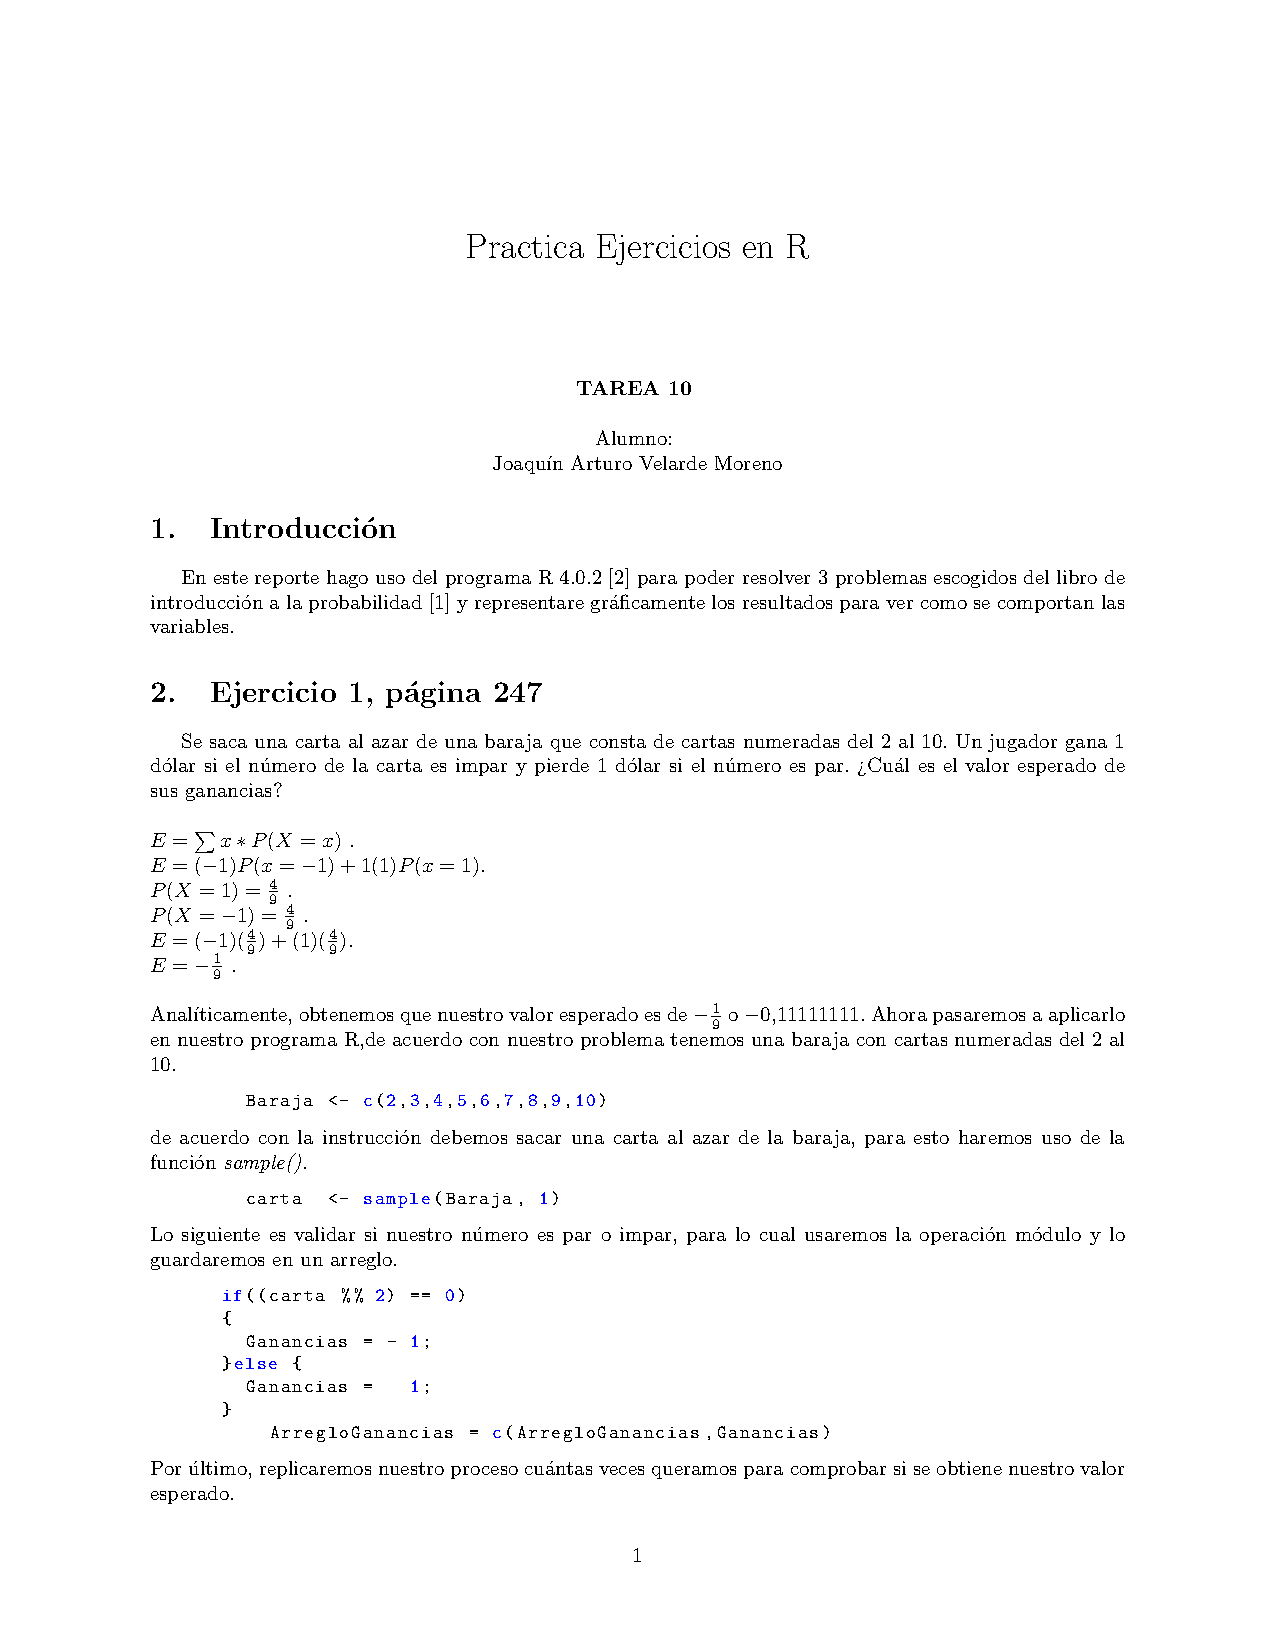
\includepdf[pages=-]{Tareas/Reporte_10.pdf}

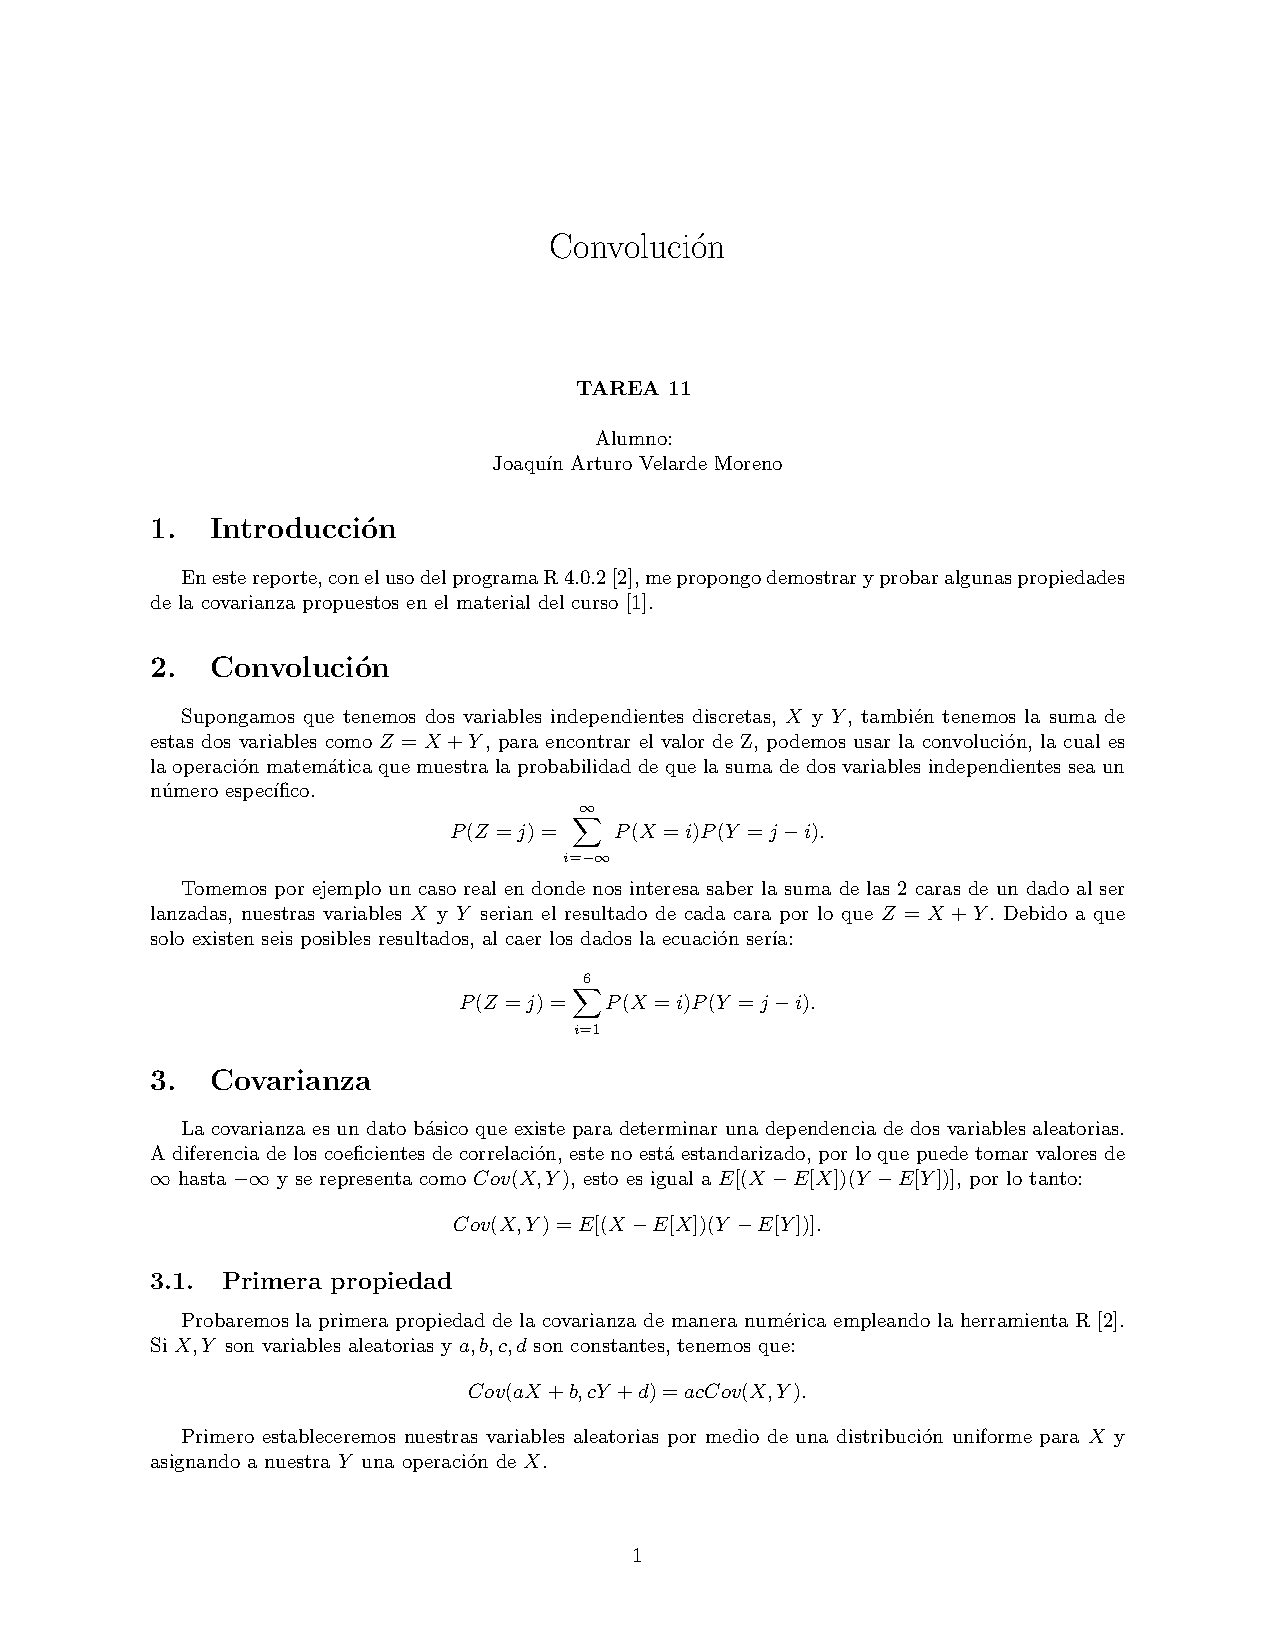
\includepdf[pages=-]{Tareas/Reporte_11.pdf}


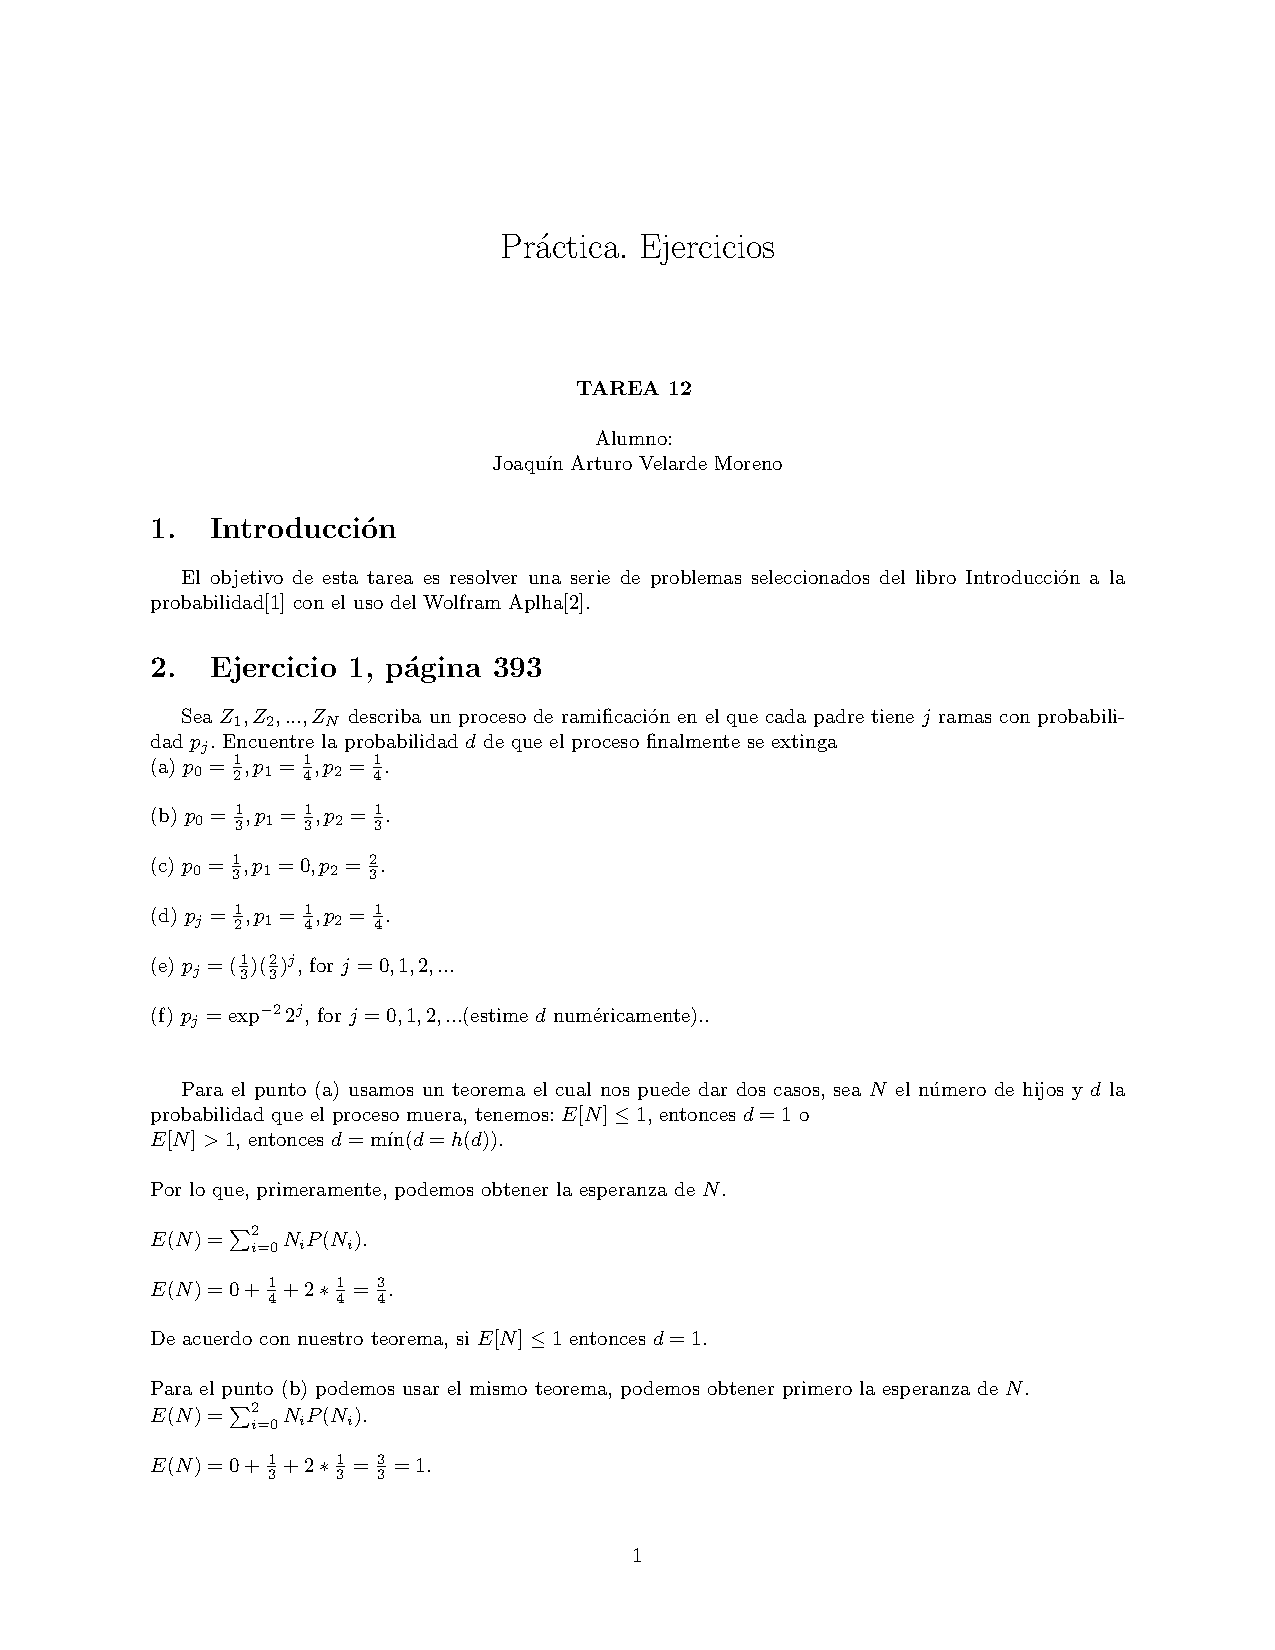
\includepdf[pages=-]{Tareas/Reporte_12.pdf}

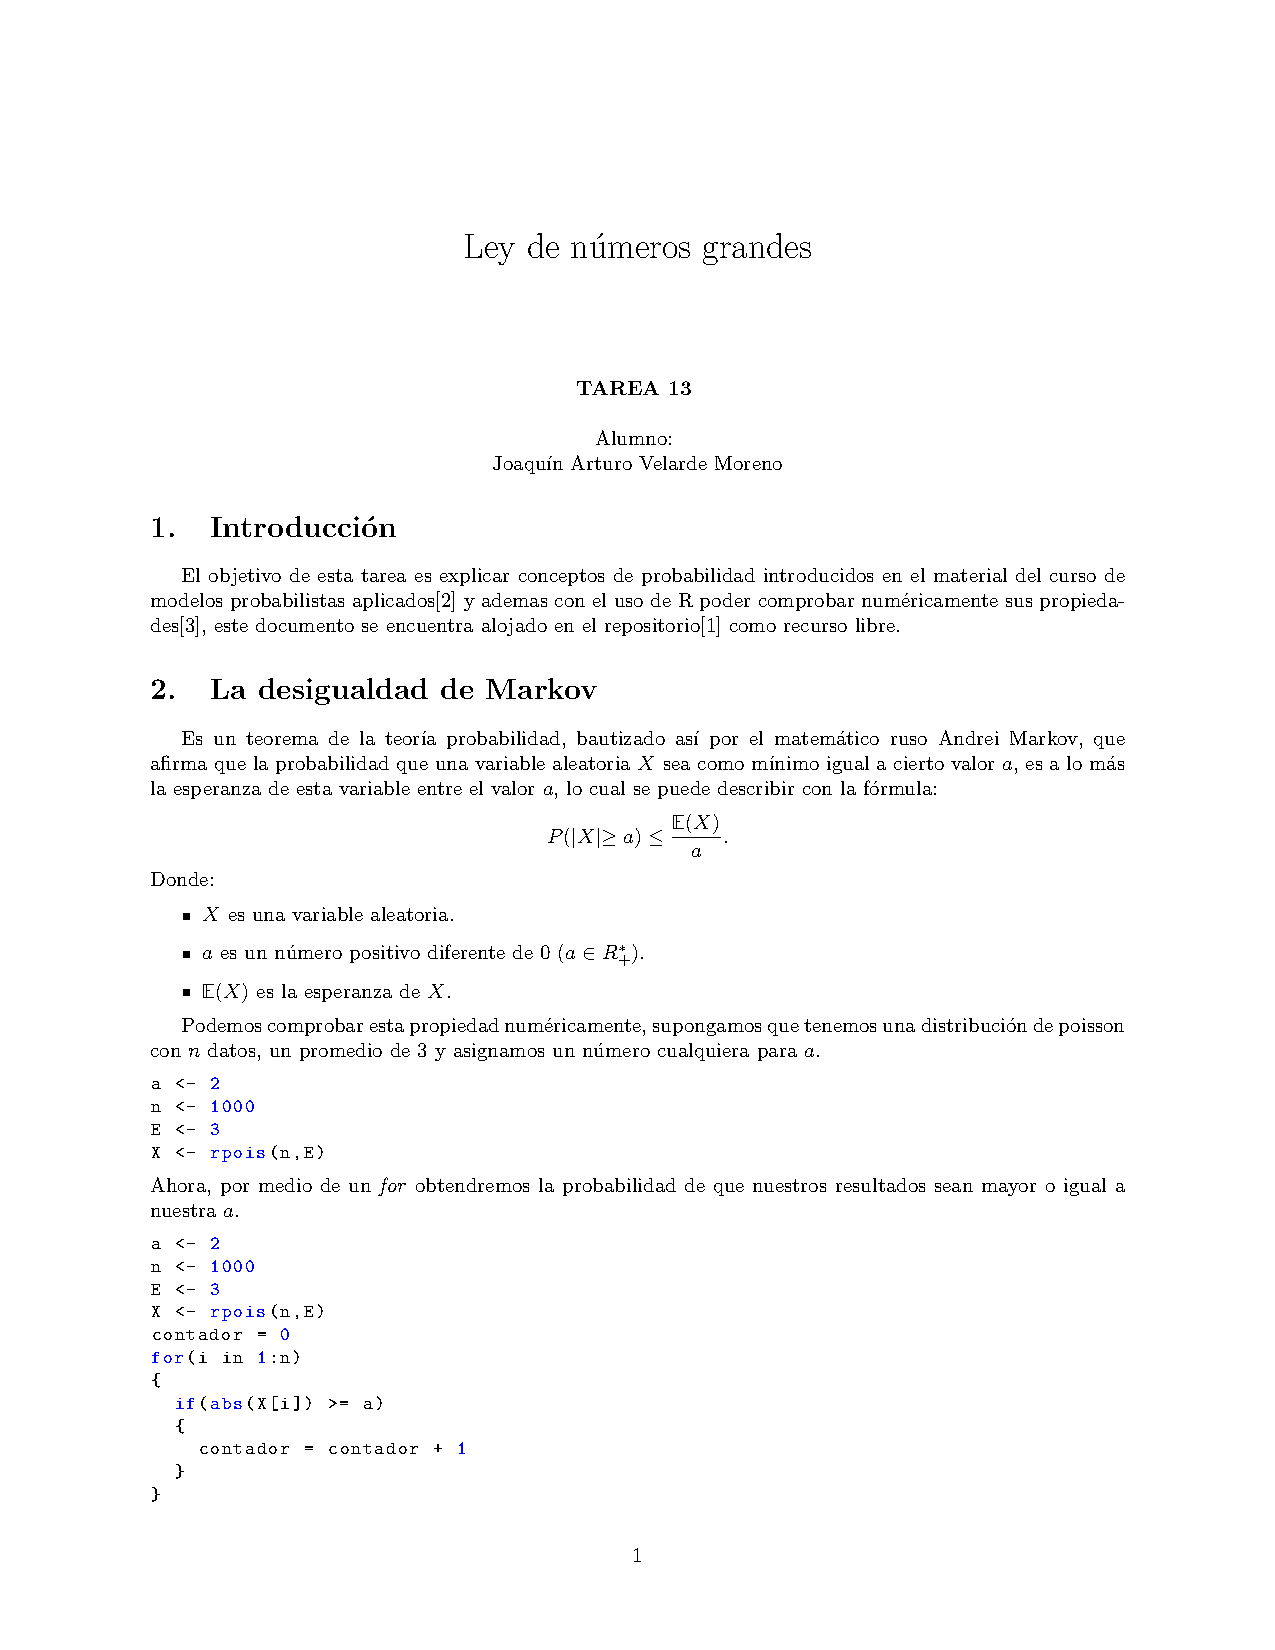
\includepdf[pages=-]{Tareas/Reporte_13.pdf}

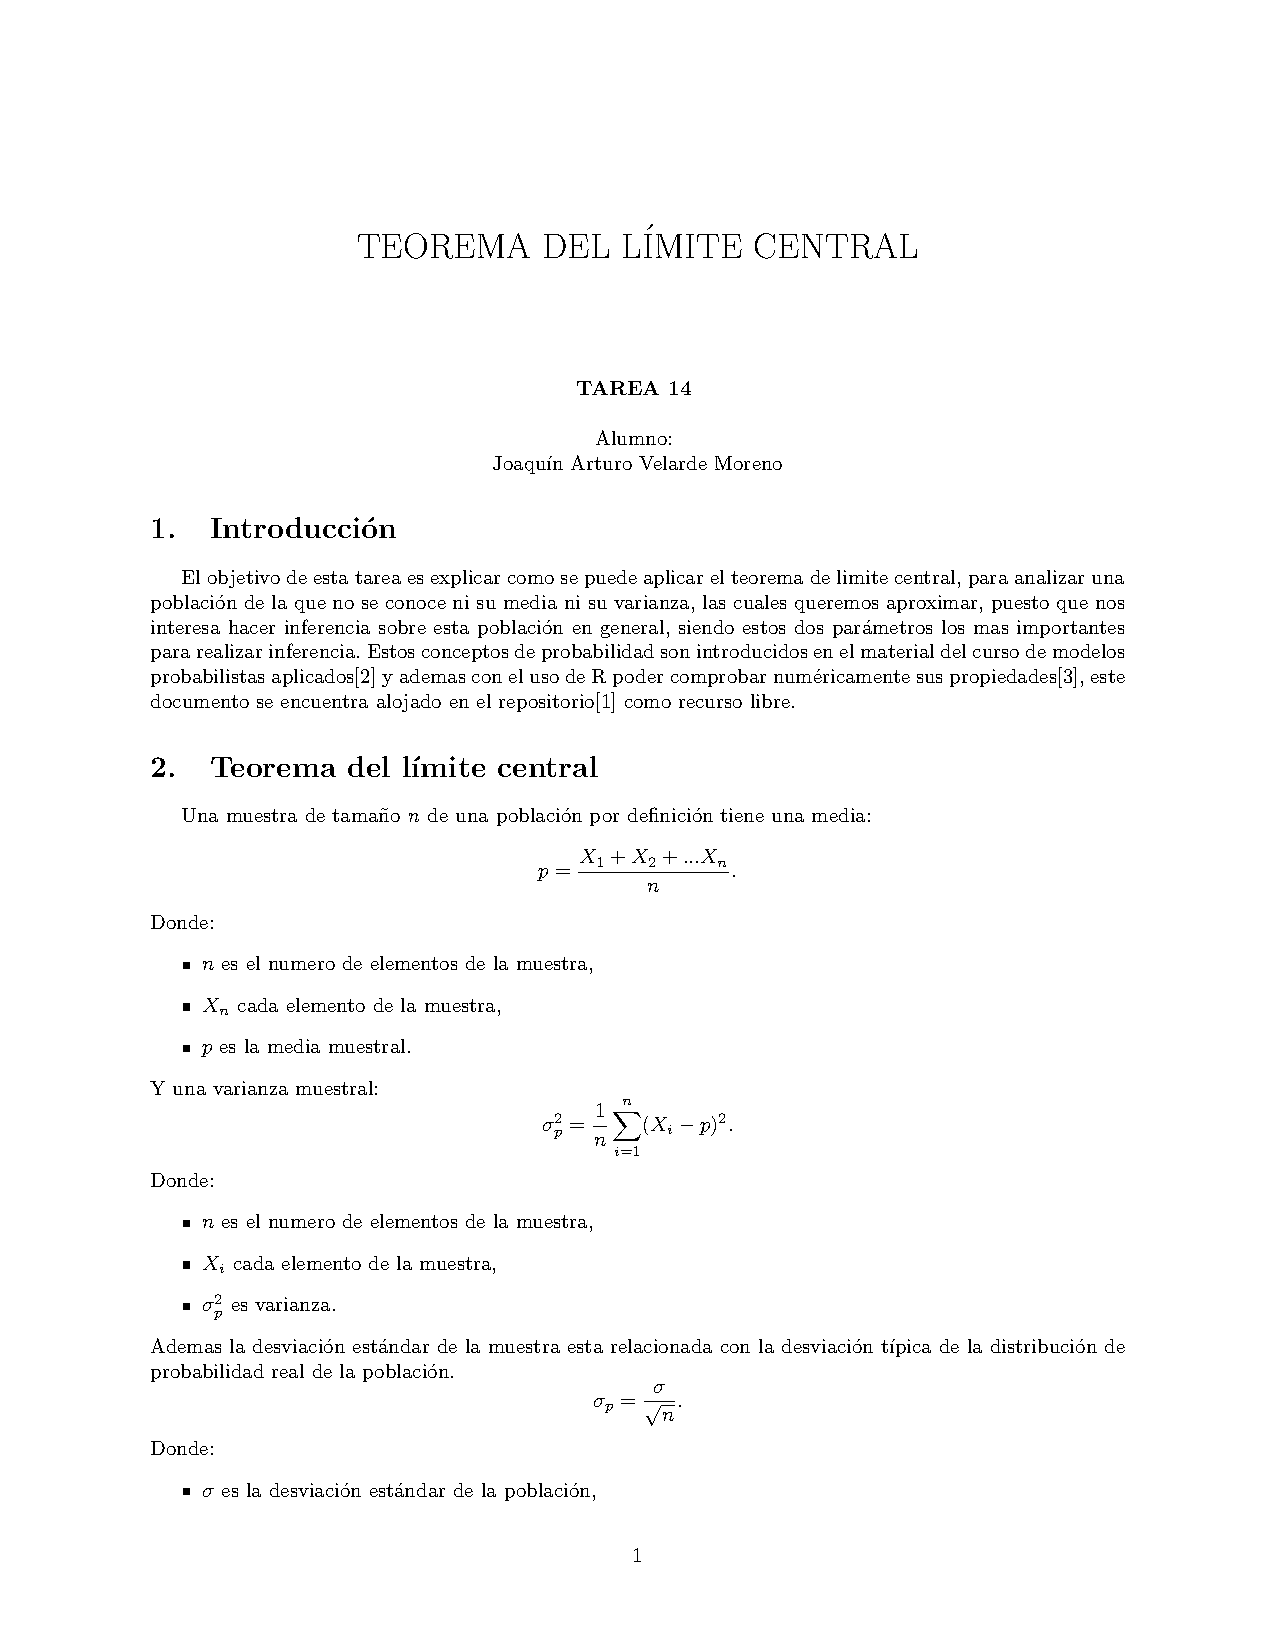
\includepdf[pages=-]{Tareas/Reporte_14.pdf}

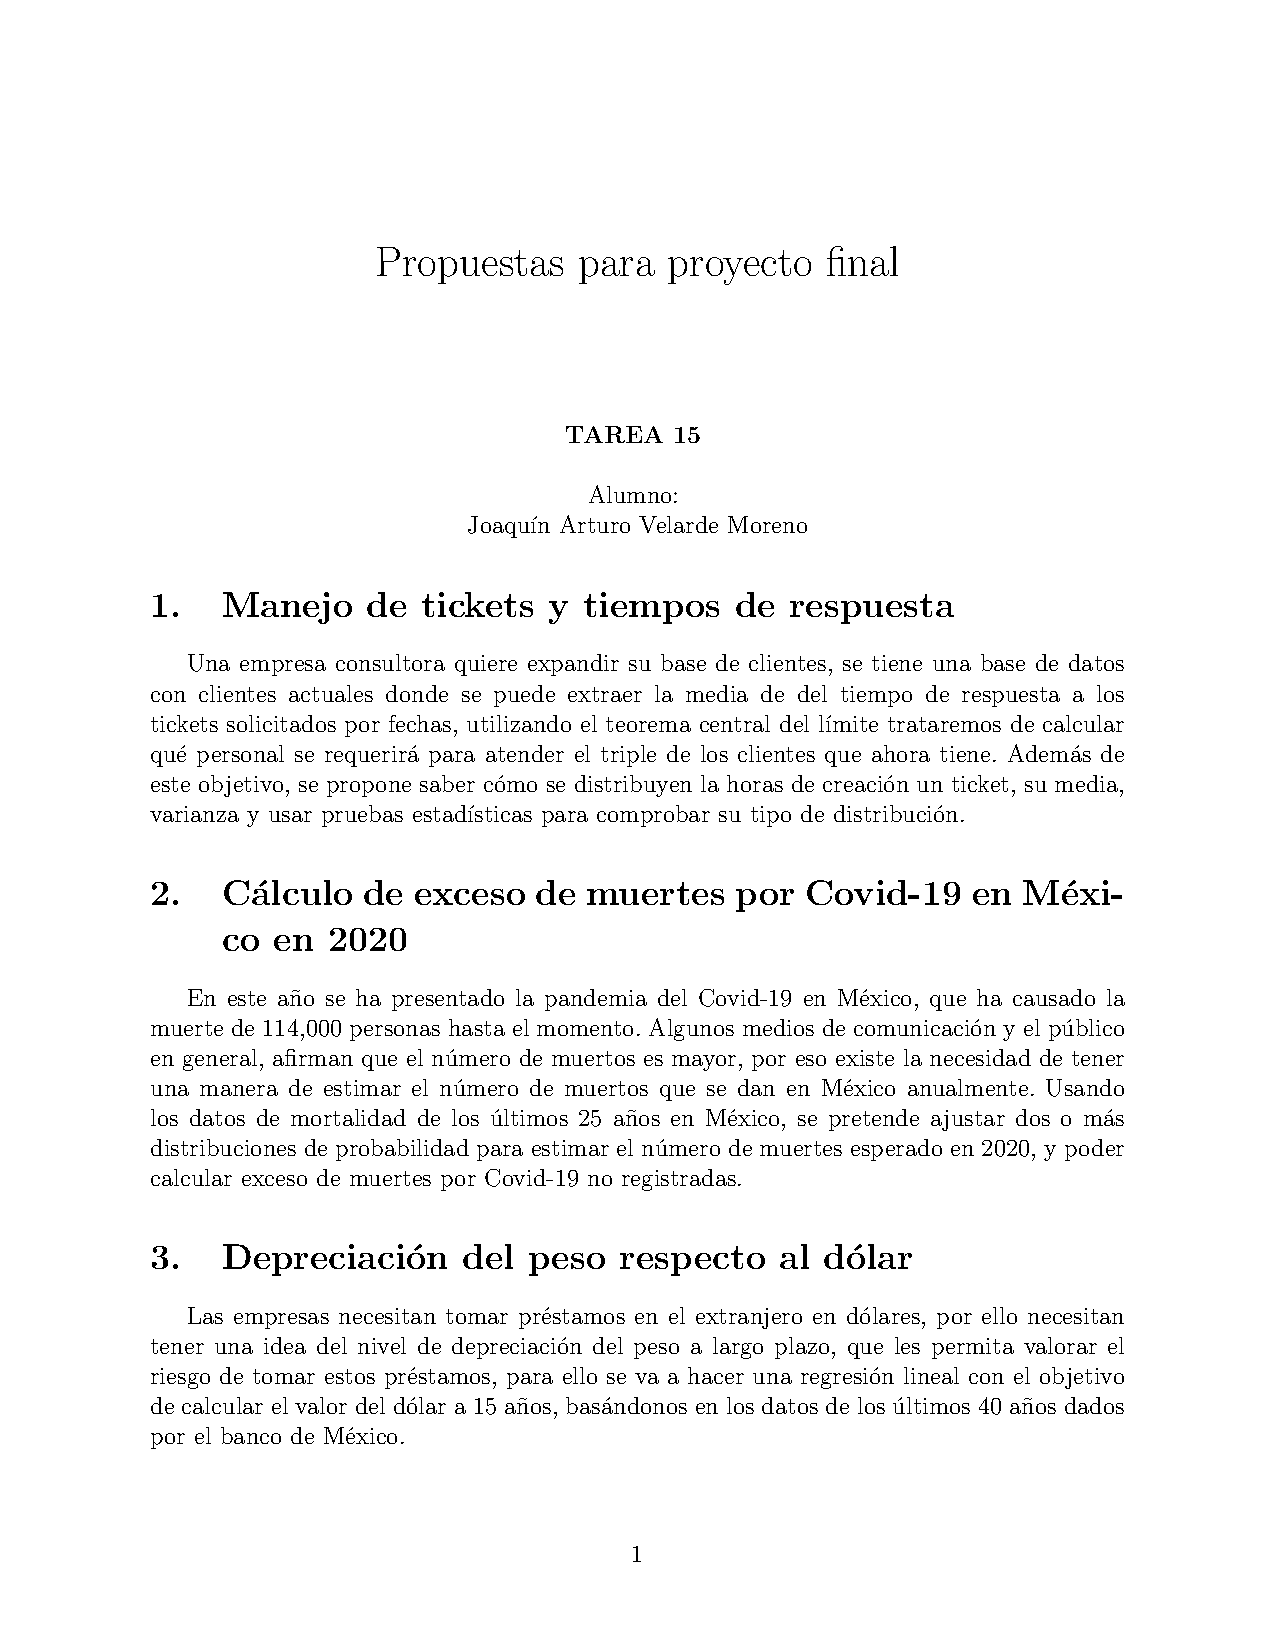
\includepdf[pages=-]{Tareas/Reporte_15.pdf}

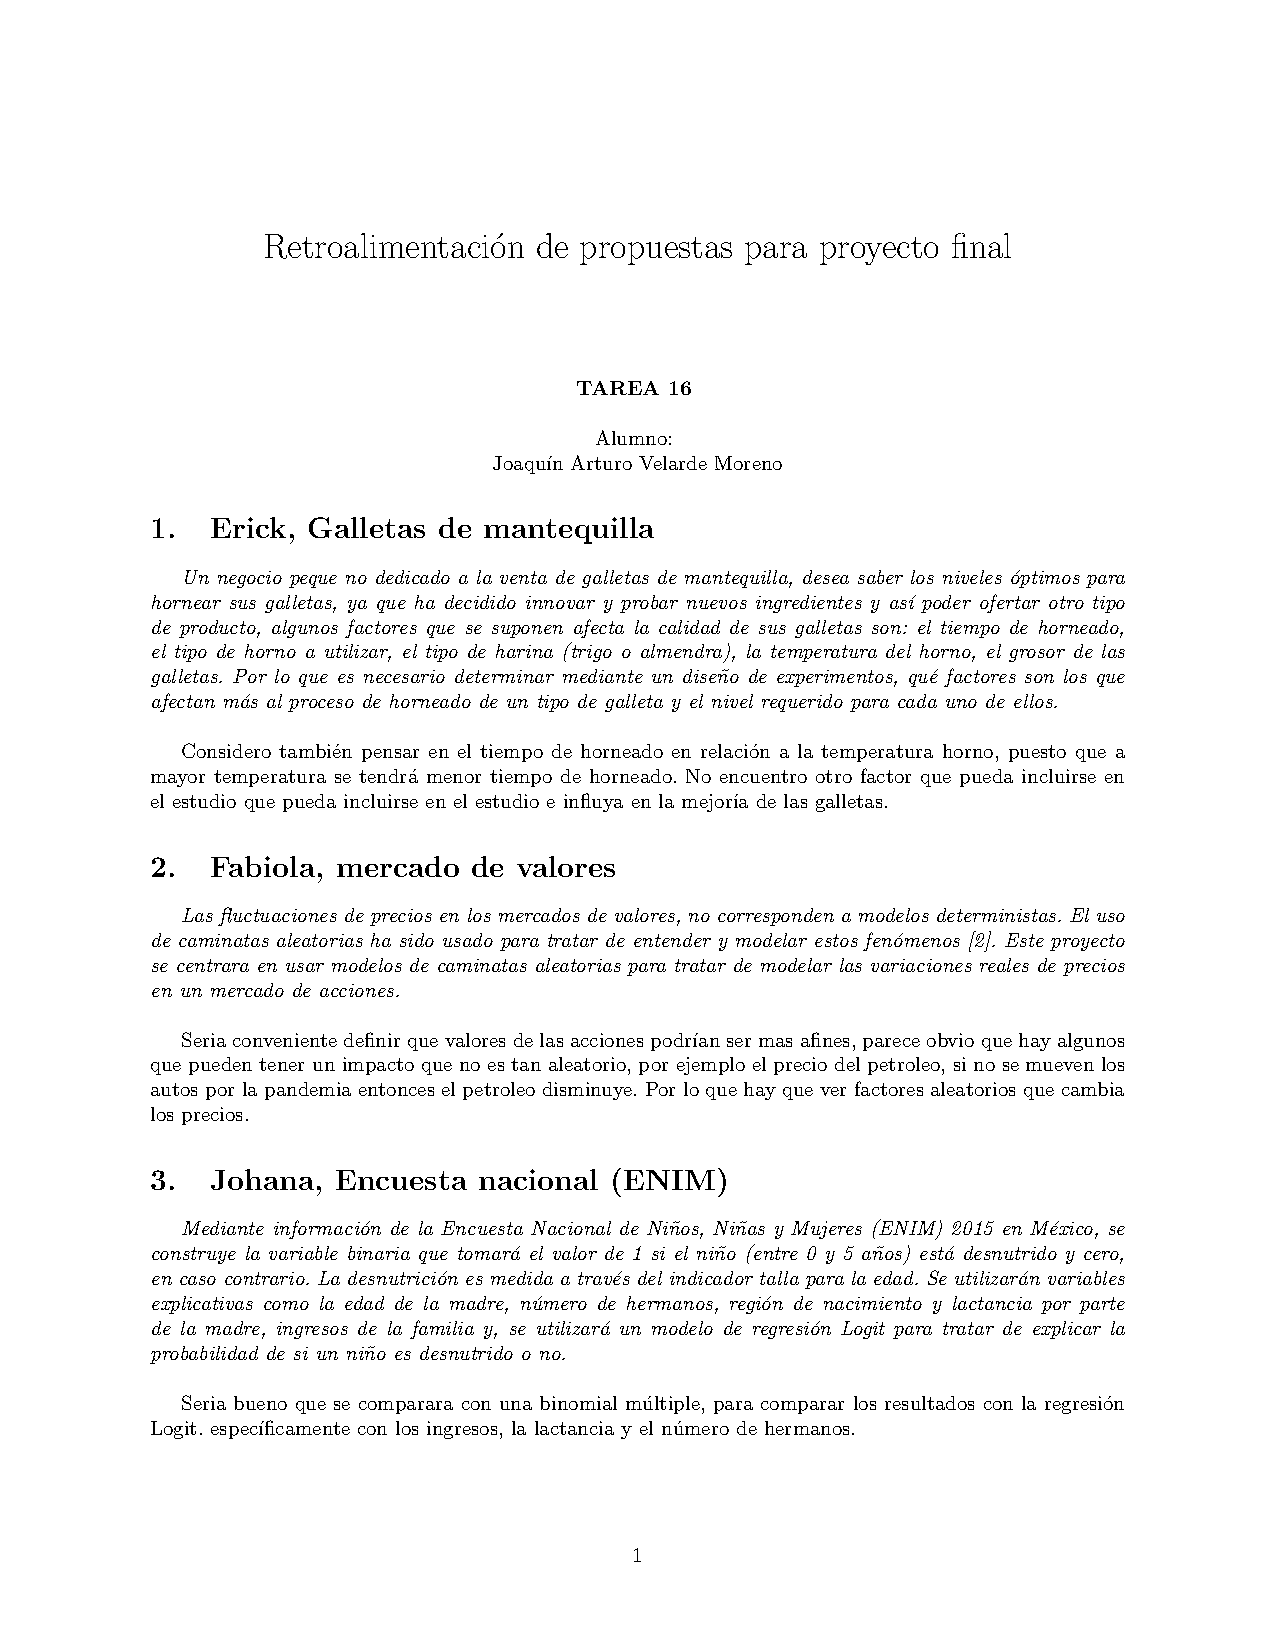
\includepdf[pages=-]{Tareas/Reporte_16.pdf}


\end{document}
